\section{Experimental Apparatus}
\label{sec:exp apparatus}

\begin{figure*}
\begin{center}
% TODO: this plot needs updating -- 210-fr unit is used
% TODO: indicate clearly (colours) the RPs used for 2-RP and 4-RP analysis
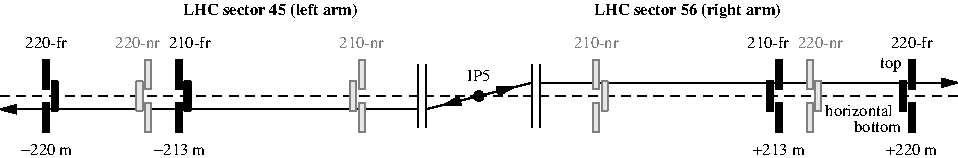
\includegraphics{fig/elastic_principle.pdf}
\hfil
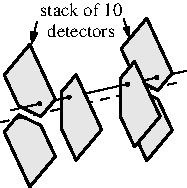
\includegraphics{fig/stationScheme.pdf}
\caption{%
Left: schematic view of the RP stations on both sides of IP5 with two proton tracks from an elastic event. Right: Schematic view of the silicon detector positions in a RP station. In the figure a track traverses the overlap zone between top and horizontal detectors, thus providing detector alignment information. 
}
\label{fig:rpsketch}
\end{center}
\end{figure*}

The TOTEM experiment, located at the LHC Interaction Point (IP) 5 together with the CMS experiment, is dedicated to the measurement of the total cross-section, elastic scattering and diffractive processes. The experimental apparatus, symmetric with respect to the IP, detect particles at different scattering angles in the forward region: a forward proton spectrometer composed of detectors in Roman Pots (RPs) and the magnetic elements of the LHC and, to measure at larger angles, the forward tracking telescopes T1 and T2. A complete description of the TOTEM detector instrumentation and its performance is given in~\cite{totem-jinst} and~\cite{totem-ijmp}. The data analysed here come from the RPs only. 

A RP is a movable beam-pipe insertion that houses the tracking detectors that are thus capable of approaching the LHC beam to a distance of less than a millimetre, and to detect protons with scattering angles of only a few microradians. The proton spectrometer is organised in two RP stations: one on the left side of the IP (LHC sector 45) and one on the right (LHC sector 56), see Figure~\ref{fig:rpsketch} (left). Each RP station, located between $215$ and $220\un{m}$ % TODO: this needs updating: 210-fr and 220-fr units are used
from the IP at the end of the straight section after the machine quadrupoles, is composed of two units: ``near'' (215\,m from the IP) and ``far'' (220\,m). A unit consists of 3 RPs, one approaching the outgoing beam from the top, one from the bottom, and one horizontally. Each RP houses a stack of 5 ``U'' and 5 ``V'' silicon strip detectors, where ``U'' and ``V'' refer to two mutually perpendicular strip orientations. The special design of the sensors is such that the insensitive area at the edge facing the beam is only a few tens of micrometers. Due to the $5\un{m}$ % TODO: this might need updating
 long lever arm between the near and the far RP units the local track angles can be reconstructed with a precision of about $10\un{\mu rad}$. % TODO: this might need updating
A high trigger efficiency ($> 99\un{\%}$) is achieved by using all RPs independently. % TODO: check what was the real trigger, TODO: move to a more appropriate place?
Since elastic scattering events consist of two collinear protons emitted in opposite directions, the detected events can have two topologies, called diagonals: 45 bottom -- 56 top and 45 top -- 56 bottom.

This article uses a reference frame where $x$ denotes the horizontal axis (pointing out of the LHC ring), $y$ the vertical axis (pointing against gravity) and $z$ the beam axis (in the clockwise direction).
